\documentclass[10pt,legalpaper]{beamer}
\usetheme{Berlin}
\usepackage{hyperref}
%\usecolortheme{spruce}
\usefonttheme{serif}
\usepackage{float}
\usepackage[natbib=true,style=authoryear,backend=bibtex,useprefix=true]{biblatex}
\addbibresource{Bibliografia.bib}
\usepackage{setspace}
\usepackage{listings}
\definecolor{backcolour}{rgb}{0.95,0.95,0.92}
\lstdefinestyle{consola}
{basicstyle=\scriptsize\bf\ttfamily,
backgroundcolor=\color{gray75},
}
\lstdefinestyle{mystyle}
{
  language=[LaTeX]{TeX},
  texcsstyle=*\color{blue},
  breaklines=false;
	number=none;
	tabsize=2;
  basicstyle=\ttfamily\footnotesize,
  keywordstyle=\color{magenta},
  commentstyle=\itshape\color{purple!40!black},
  identifierstyle=\color{blue},
  backgroundcolor=\color{gray!10!white},
  moretexcs={mycommand}, % user command highlight
  frame=single,
}
\setbeamersize{text margin left=8mm,text margin right=5mm}
\setbeamertemplate{footline}[page number]
\setbeamertemplate{headline}{}
\setbeamertemplate{background}{
\includegraphics[width=\paperwidth,height=\paperheight]{FondoUNAH}}
\usepackage[utf8]{inputenc}
\usepackage{float}
\usepackage[spanish]{babel}
\usepackage{amsmath}
\usepackage{mathtools}
\usepackage{multicol}
\usepackage{amsfonts}
\usepackage{amssymb}
\usepackage{xcolor}
\usepackage{color}
\usepackage{graphicx}
\renewcommand{\indent}{\hspace*{2em}}
\hypersetup{
    bookmarks=true,         % show bookmarks bar?
    unicode=false,          % non-Latin characters in Acrobat’s bookmarks
    pdftoolbar=true,        % show Acrobat’s toolbar?
    pdfmenubar=true,        % show Acrobat’s menu?
    pdffitwindow=false,     % window fit to page when opened
    pdfstartview={FitH},    % fits the width of the page to the window
    pdftitle={My title},    % title
    pdfauthor={Author},     % author
    pdfsubject={Subject},   % subject of the document
    pdfcreator={Creator},   % creator of the document
    pdfproducer={Producer}, % producer of the document
    pdfkeywords={keyword1, key2, key3}, % list of keywords
    pdfnewwindow=true,      % links in new PDF window
    colorlinks=false,       % false: boxed links; true: colored links
    linkcolor=red,          % color of internal links (change box color with linkbordercolor)
    citecolor=green,        % color of links to bibliography
    filecolor=cyan,         % color of file links
    urlcolor=magenta        % color of external links
}
\author{Myrian Gonzalez Orellana}
\title{Departamento de Matemática Aplicada\\
Análisis Numérico, MM412}
\institute{UNAH} 
\date{PACIII2023}  
\begin{document}
\setstretch{0.7}
\begin{frame}
\titlepage
\end{frame}
\begin{frame}{\centering\textbf{Tabla de Contenidos}}
\tableofcontents[hideallsubsections]
\end{frame}
%Primera Unidad
\section{Preliminares del cálculo}
\begin{frame}[allowframebreaks]{Teoremas Preliminares}
Esta presentación esta basada en el texto de \textcolor{gray}{\cite{burden2017análisis}}.
\label{RetornoTeoremaPreliminares1}
\begin{block}{Criterio del límite}
Sea $f:\mathbb{R}:\rightarrow \mathbb{R}$. Asuma que $\lim_{x\rightarrow \infty}f(x)$ existe y es igual a $L$. Entonces la sucesión $\{a_n\}=\{f(n)\}$ converge a $L$ también.  
\end{block}
\hyperlink{CriterioLimite}{\textcolor{cyan}{Enlace a ejercicio.}}
\begin{block}{Teorema de convergencia monótona}
Suponga que la sucesión $\{a_n\}$ es monótona creciente y acotada superiormente, entonces $\{a_n\}$ es convergente.
\end{block}
\hyperlink{ConvergenciaMonotona}{\textcolor{cyan}{Enlace a ejercicio.}}
\begin{block}{Teorema del sándwich}
Suponga que $\{a_n\}$ y $\{b_n\}$ convergen al valor de $L$. Además asuma que
$$a_n\leq x_n\leq b_n,$$
para $n>N$ para algún $N$ fijo; entonces $\{x_n\}$ converge a $L$.
\end{block}
\hyperlink{Sandwich}{\textcolor{cyan}{Enlace a ejercicio.}}
\framebreak
\label{RetornoTeoremaPreliminares2}
\begin{block}{Teorema del valor medio}
Si $f\in C[a,b]$ y $f$ es diferenciable en $(a,b),$ entonces existe un número $c$ en $(a,b)$ con
$$f'(c)=\dfrac{f(b)-f(a)}{b-a}.$$
\end{block}
\begin{figure}[H]
\begin{center}
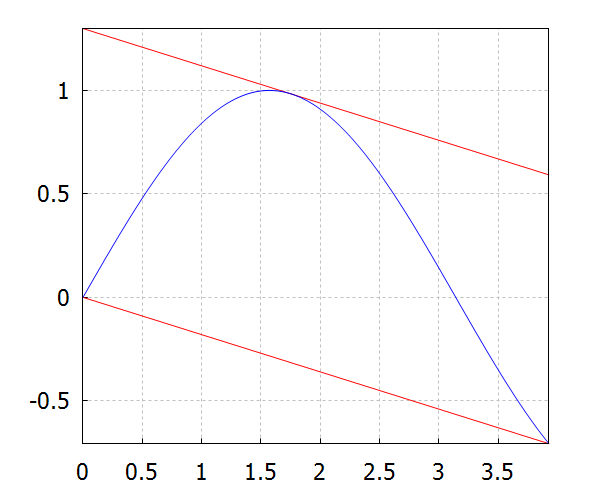
\includegraphics[scale=0.5]{Imagen17}
\end{center}
\caption{En la figura se puede ver un ejemplo con $f(x)=\sin(x)$ para $x\in \bigg[0,\dfrac{5\pi}{4}\bigg]$}
\end{figure}
\framebreak
\vspace*{-0.7cm}
\label{RetornoTeoremaPreliminares3}
\begin{block}{Teorema del valo extremo}
\begin{itemize}
\item Si $f\in C[a,b]$, entonces existe $c_1,c_2\in [a,b]$ con
$$f(c_1)\leq f(x)\leq f(c_2)$$
para $x\in[a,b]$.
\item Si además $f$ es diferenciable en $(a,b)$, entonces $c_1$ y $c_2$ son iguales a los extremos ($a$ o $b$) o los lugares donde la derivada se hace cero en $(a,b)$. 
\end{itemize}
\hyperlink{EjercicioExtremos}{\textcolor{cyan}{Enlace a ejercicio}}
\end{block}
\begin{figure}[H]
\begin{center}
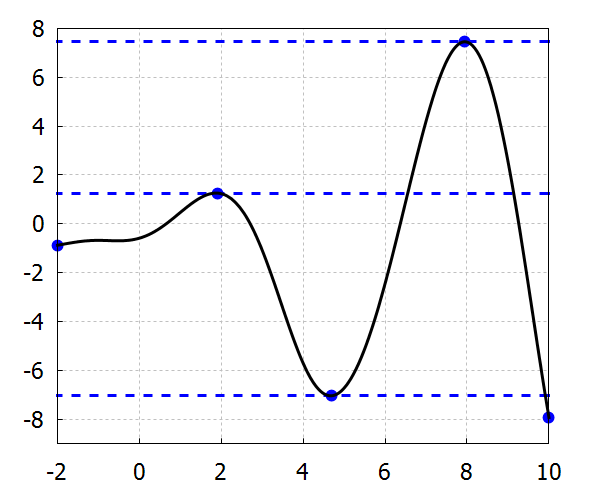
\includegraphics[scale=0.4]{Imagen18}
\end{center}
\caption{Se puede apreciar en el ejemplo, que el máximo de la función se alcanza en un lugar donde la derivada es cero y el mínimo en el extremo derecho.}
\end{figure}
\framebreak
\label{RetornoTeoremaPreliminares4}
\begin{block}{Teorema del valor intermedio}
Si $f\in C[a,b]$ y $K$ es cualquier número entre $f(a)$ y $f(b)$, entonces existe un número $c$ en $(a,b)$ para el cual $f(c)=K$.
\end{block}
\hyperlink{EjercicioIntermedio}{\textcolor{cyan}{Enlace a ejercicio}}
\begin{figure}[H]
\begin{center}
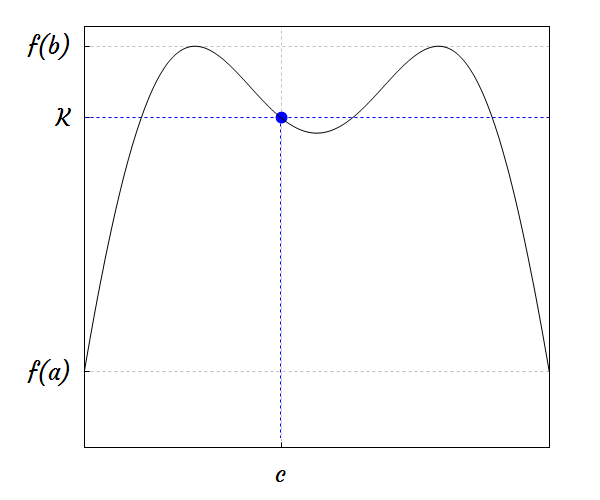
\includegraphics[scale=0.7]{Imagen19}
\end{center}
\end{figure}
\framebreak
Se define $C^n[a,b]=\{f:[a,b]\rightarrow \mathbb{R}| f,f',\cdots,f^{(n)}\text{ son continuas en }[a,b]\}.$
\label{RetornoTeoremaPreliminares5}
\begin{block}{Teorema de Taylor}
Supong que:
\begin{itemize}
\item $f\in C^n[a,b]$.
\item $f^{(n+1)}$ esta definida en $[a,b]$.
\item $x_0\in[a,b]$.
\end{itemize} 
Entonces, para cada $x\in[a,b]$, existe $\xi(x)\in (x_0,x)$ (si $x>x_0$ y $\xi(x)\in(x,x_0)$ en el otro caso)  tal que: 
\begin{itemize}
\item $f(x)=P_n(x)+R_n(x)$ donde
\item $P_n(x)=\displaystyle \sum_{k=0}^{n}\dfrac{f^{(k)}(x_0)}{k!}(x-x_0)^k$ y
\item $R_n(x)=\dfrac{f^{(n+1)}(\xi(x))}{(n+1)!}(x-x_0)^{(n+1)}$.
\end{itemize}
\end{block}
\hyperlink{EjercicioTaylor}{\textcolor{cyan}{Enlace a ejercicio}}
\end{frame}
\section{Raíces de ecuaciones}
\begin{frame}[allowframebreaks,fragile]{Raíces de ecuaciones}
\label{RetornoTeoremaRaices1}
\begin{figure}[H]
\begin{center}
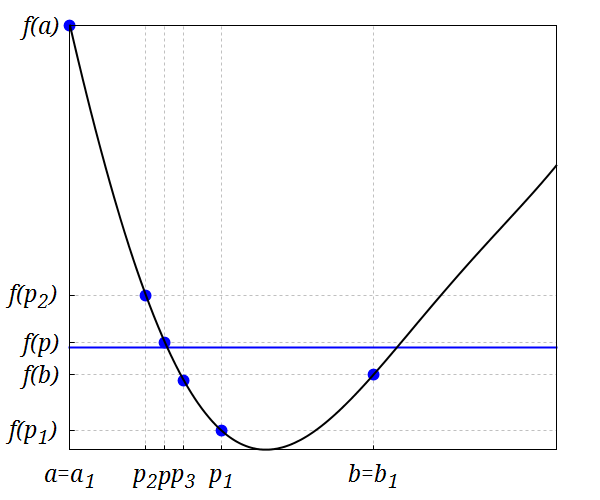
\includegraphics[scale=0.7]{Imagen20}
\end{center}
\caption{\textbf{Método de Bisección: }En la figura se muestra el mécanismo de la bisección.}
\end{figure}
\label{RetornoTeoremaRaices2}
\begin{lstlisting}[caption=''Método de Bisección'',style=mystyle,language=octave,numbers=left]
function x=Biseccion(f,a,b,TOL,N0)
  i=1;FA=f(a);
  while(i<=N0)
    p=a+(b-a)/2;
    FP=f(p);
    if(FP==0 || (b-a)/2<TOL)
      x=p;
      break;
    endif
    i=i+1;
    if(FA*FP>0) 
      a=p;
      FA=FP;
    else
      b=p;  
    endif
  endwhile
  if(i>N0)
    x=inf;
  endif
endfunction
\end{lstlisting}
\label{RetornoTeoremaRaices3}
\begin{block}{Teorema de convergencia del método de bisección}
Supongamos que $f\in C[a,b]$ y $f(a)f(b)<0$. El método de bisección genera una sucesión $\{p_n\}$ que aproxima a un cero de $p$ de $f$, tal que:
$$|p_n-p|\leq \dfrac{b-a}{2^n}.$$
\hyperlink{EjercicioBiseccion}{\textcolor{cyan}{Enlace a ejercicio}}
\end{block}
\textcolor{red}{
\indent Primero note que $p\in [a_n,b_n]$ (teorema del valor intermedio), entonces $$|p-(a_n+b_n)/2|\leq(b_n-a_n)/2.$$ De esto se tiene que:
\begin{align*}
|p_n-p|=&|(a_n+b_n)/2-p|\\
\leq & \dfrac{b_n-a_n}{2}\\
\leq & \dfrac{1}{2}\dfrac{b-a}{2^{n-1}} (\text{ inducción}: b_n-a_n\leq \dfrac{b-a}{2^{n-1}})\\
=& \dfrac{b-a}{2^n.}
\end{align*}
}
\label{RetornoTeoremaRaices4}
\begin{block}{Iteración de Newton Raphson}
La iteración de Newton Rapshon se define como:
$$p_{n+1}=p_n-\dfrac{f(p_n)}{f'(p_n)}.$$
La sucesión $\{p_n\}$ intenta resolver el problema:
$$f(x)=0.$$
\end{block}
\indent Como se suele encontrar en muchos textos y con justa razón, el método de Newton-Raphson \footnotetext{\vspace*{-1cm}La razón por la que aparece Raphson aparece en el nombre del método es poque Joseph Raphson publicó el método de forma independiente a Newton y lo hizo más temprano también.} es uno de los métodos más poderosos conocidos para la resolución de ecuaciones. \\
\indent Idea detrás del método: Suponga que se quiere investigar como resolver la ecuación:
$$f(x)=0$$
\indent Supogan además que la raíz a esta ecuación sucede en $x=p.$ Por el teorema de Taylor bajo algunas suposiciones tenemos que:
$$0=f(p)=f(x)+(p-x)f'(x)+\dfrac{(p-x)^2}{2}f''(\xi)$$
\indent Si se asume que $x$ está cerca de $p$ entonces, después de despejar arriba se tiene:
$$p\approx x-\dfrac{f(x)}{f'(x)},\ (p-x)^2\approx 0.$$
\indent Esto último, como se puede notar, tiene la estructura de la iteración del método de Newton presentada al inicio.\\
\indent El método iterativo de Newton se puede analizar desde el teorema de punto fijo; para ello considere primero el enunciado de dicho teorema:
\framebreak
\begin{block}{Teorema de punto fijo}
Suponga lo siguiente:
\begin{itemize}
\item $g\in C[a,b].$
\item $g(x)\in[a,b].$
\item Suponga que $g'$ existe en $(a,b)$.
\item Existe una constante positiva $k$ menor que 1 tal que $|g'(x)|\leq k$
para toda $x\in (a,b).$
\end{itemize}
Entonces para cualquier $p_0\in[a,b]$ la sucesión definida por $p_n=g(p_{n-1})$ converge al único punto fijo $p$ tal que $$p=g(p).$$
\end{block}
\indent En la iteración de Newton, $g(x)=x-\dfrac{f(x)}{f'(x)}$; si se asume que $f'(p)\neq 0$ y cumple con todas las condiciones del teorema de punto fijo, entonces la conclusión de este es que la sucesión converge a $p$ y
$$p=g(p)=p-\dfrac{f(p)}{f'(p)},$$
esto deriva en que $f(p)=0$; lo que justamente se anda buscando.\\
\indent Para que se garantice el teorema de punto fijo, se tiene el siguiente teorema sobre el método de Newton:
\begin{block}{Teorema de convergencia del método de Newton}
Suponga que:
\begin{itemize}
\item $f\in C^2[a,b]$.
\item $p\in [a,b]$.
\item $f(p)=0$, $f'(p)\neq 0.$
\end{itemize}
Entonces existe un $\delta>0$ tal que la sucesión $\{p_n\}$ converge a $p$ para cualquier aproximación inicial $p_0\in [p-\delta,p+\delta].$
\end{block}
\indent La demostración del teorema se puede encontrar en \textcolor{gray}{\cite{burden2017análisis}}. En el podrás observar que se usa el teorema de punto fijo.\\ 
\indent Para apreciar la importancia del método de Newton, se necesita la siguiente definición:
\framebreak
\begin{block}{Orden de convergencia}
Suponga que $\{p_n\}$ es una sucesión que converge a $p$ y que $p\neq p_n$ para toda $n$. Además asuma que existen constantes positivas $\lambda$ y $\alpha$ tales que:
$$\lim_{n\rightarrow \infty}\dfrac{|p_{n+1}-p|}{|p_n-p|^\alpha}=\lambda.$$
entonces se dice que:
\begin{itemize}
\item $\alpha$ es le orden de convergencia de la sucesión $\{p_n\}$.
\item $\gamma$ es la constante de error asintótica.
\end{itemize} 
\end{block}
\indent A conitinuación se hacen algunas observaciones:
\begin{itemize}
\item La parte más relevante en la definición anterior es el orden de convergencia $\alpha$; entre más grande sea este, el método convergerá con mayor rapidez.
\item El método de bisección tiene un orden de convergencia $\alpha=1$ (esto se denomina convergencia  lineal).
\item Bajo ciertos supuestos razonables, el método de Newton posee una convergencia de al menos $\alpha=2$ (esto se denomina convergencia  cuadrática). Debido a su valor en el orden de convergencia, a este método se le considera de rápida convergencia.
\item Usualemente se preferirá el método de Newton sobre el método de bisección; sin embargo hay que notar que la desventaja del método de Newton es la escogencia del valor inicial y una combinación de ambos métodos es en general la mejor opción.
\end{itemize}
\hyperlink{EjercicioNewton}{\textcolor{cyan}{Enlace a ejercicio}}
\framebreak
\label{RetornoTeoremaRaices10}
\begin{block}{Sistema de ecuaciones}
Un sistema de ecuaciones, en general tiene la siguiente forma:
\begin{displaymath}
\begin{bmatrix}
f_1(x_1,\cdots ,x_n)=0\\
f_2(x_1,\cdots ,x_n)=0\\
\vdots\\
f_n(x_1,\cdots ,x_n)=0
\end{bmatrix}
\end{displaymath}
El cual se puede expresar de forma compacta como:
$$F(X)=0,$$
donde $X=[x_1,\cdots,x_n]$ y $F(X)=[f_1(X),\cdots,f_n(X)].$
\end{block}
\indent Todo el análisis que se hizo antes en el caso de una variable, se puede hacer para el caso en el que queremos resolver un sistema de ecuaciones.\\[2cm]
\small
\begin{block}{Iteración del método de Newton para sistemas}
Se define la iteración de Newton para sistemas como:
$$p_{n+1}=p_{n}-J^{-1}(p_{n})F(p_{n}),$$
donde:
\begin{align*}
J(x)=&
\begin{pmatrix}
\dfrac{\partial f_1(X)}{\partial x_1} & \cdots & \dfrac{\partial f_1(X)}{\partial x_n}\\
\vdots &\vdots &\vdots\\
\dfrac{\partial f_n(X)}{\partial x_1} & \cdots & \dfrac{\partial f_n(X)}{\partial x_n}\\
\end{pmatrix}\\
=&
\begin{pmatrix}
\bigtriangledown f_1(X)\\
\vdots\\
\bigtriangledown f_n(X)
\end{pmatrix}\\
p_{n}\in &\mathbb{R}^n
\end{align*}
\end{block}
\indent A $J$ se le conoce como el jacobiano en la literatura.\\
\indent Para medir los errores en el caso de sistemas, en lugar del valor absoluto se usa su equivalente, las normas. Las normas que se suelen usar son las siguientes:
\begin{itemize}
\item Norma 2: $\parallel x\parallel_2=\sqrt{x_1^2+\cdots +x_n^2}$.
\item Norma 1: $\parallel x\parallel_1=|x_1|+\cdots +|x_n|$.
\item Norma infinito: $\displaystyle \parallel x\parallel_\infty=\max_{1\leq i\leq n}|x_i|$.
\end{itemize}
\indent Por ejemplo, si se quiere medir el error entre la aproximación $p_n$ de $p$, donde estos son vectores, entonces:
\begin{itemize}
\item Error absoluto en la norma infinito: $\displaystyle \parallel p-p_n\parallel_\infty$
\item Error relativo en la norma 1: $\displaystyle \dfrac{\parallel p-p_n\parallel_1}{\parallel p \parallel_1}$
\end{itemize}
\indent Cuando no se conoce el valor exacto entonces se suelen usar medidas para estimar el valor relativo o absoluto; para ello suponga que se quiere estimar el error para una suceción $\{p_n\}$ vectorial:
\begin{itemize}
\item Estimación error absoluto en la norma 2: $\displaystyle \parallel p_{n+1}-p_n\parallel_2$
\item Estimación del error relativo en la norma infinito: $\displaystyle \dfrac{\parallel p_{n+1}-p_n\parallel_\infty}{\parallel p_{n+1} \parallel_\infty}$
\end{itemize}
\hyperlink{EjercicioNewtonSistemas}{\textcolor{cyan}{Enlace a ejercicio}}
\end{frame}
%%Segunda Unidad
\begin{frame}{Teoremas preliminares}
\begin{block}{Teorema de Weierestrass}
Suponga que $f$ está definida y es continua en $[a, b]$. Para cada $\epsilon>0$, existe un polinomio $P(x)$, con la propiedad de que 
$$|f(x)-P(x)|<\epsilon, \quad \forall x \in [a, b]$$
\end{block}
\end{frame}

%===========================
\begin{frame}{Utilidad de los polinomios para aproximar funciones}
Los polinomios son ampliamente utilizados para la interpolación numérica porque:
\begin{itemize}
\item Aproximan de manera uniforme a las funciones conitnuas. 
\item Tienen derivadas e integrales fáciles de calcular. Además, sus integrales y derivadas también son polinomios. 
\end{itemize}
\end{frame}

%===========================
\begin{frame}{Limitaciones de los polinomios de Taylor para la interpolación}
Las principales limitaciones de los polinomios de Taylor son:
\begin{itemize}
\item Generalmente no ofrecen una buena aproximación en todo un intervalo, sino que la aproximación se concentra alrededor de $x_0$.
\item Aumentar el grado del polinomio de Taylor no necesariamente brindará una mejor aproximación.   
\item No utilizan más que un único punto para definir el polonomio.  
\end{itemize}

Debido a las limitaciones expuestas, los polinomios de Taylor se usan principalmente para:
\begin{enumerate}
\item Derivación de otros métodos numéricos, como el método de diferencias finitas.
\item Estimación del error
\end{enumerate}
\end{frame}

%===========================
\begin{frame}{Polinomio interpolante de Lagrange}
\small
\begin{block}{Teorema: polinomios de Lagrange}
Si $x_0, x_1, x_2,..., x_n$ son $n+1$ números distintos y si $f$ es una función cuyos valores están dados en esos números, entonces existe un único polinomio $P(x)$ de grado a lo más $n$, con la propiedad:
$$f(x_k)=P(x_k)\quad k=0, 1, \dots, n$$
El polinomio $P(x)$ se define como sigue:
\begin{align*}
P(x)&=\sum_{k=0}^{n}f(x_k)L_{n,k}(x)\qquad k=0, 1, \dots, n\\
    &=f(x_0)L_{n,0}+f(x_1)L_{n,2}+\dots+f(x_n)L_{n,n}
\end{align*}
donde
$$L_{n,k}=\frac{(x-x_0)(x-x_1)\dots(x-x_{k+1})(x-x_{k+1})\dots (x-x_n)}{(x_k-x_0)(x_k-x_1)\dots(x_k-x_{k+1})(x_k-x_{k+1})\dots (x_k-x_n)}$$
\end{block}
\end{frame}
%===========================
\begin{frame}
\begin{block}{Término del error del polinomio de Lagrange}
Suponga que $x_0, x_1, \dots, x_n$ son números distintintos en el intervalo $[a,b]$ y que $f \in C^{n+1}[a,b]$. Entonces, para cada x en $[a,b]$ existe in número $\xi(x)$ en $(a,b)$ con 
$$f(x)=P(x)+\frac{f^{(n+1)}(\xi(x))}{(n+1)!}(x-x_0)(x-x_1)\dots (x-x_n)$$
donde $P(x)$ es el polinomio interpolante de Lagrange.
\end{block}
\end{frame}
\begin{frame}[allowframebreaks]{Interpolación, Spline Cúbicos}
\indent Considere el siguiente ajuste polinomial:
\begin{figure}[H]
\begin{center}
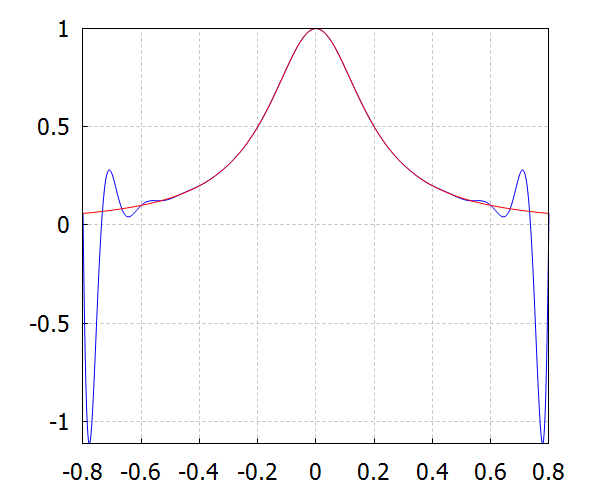
\includegraphics[scale=0.7]{Imagen21}
\end{center}
\caption{En la figura se observa la interpolación por polinomios de Lagrange para $f(x)=\dfrac{1}{1+25x^2}$ para $x\in[-1,1]$ con 30 puntos equidistante comenzando en -1 y finalizando en 1.}
\end{figure}
\indent El ejemplo anterior demuestra que los polinomios de alto orden (en el ejemplo de la figura tendríamos un polinomio de orden 31)  pueden oscilar erráticamente. Evidentemente esta característica es indeseable en muchas situaciones; en este apartado se mostrará una técnica que puede evitar este problema siempre con la idea de hacer un ajuste polinomial. \\
\indent Los ingredientes para construir un \textbf{spline} (esta palabra no tiene traducción al español, su significado es "larga tira flexible") \textbf{cúbico interpolante} $S$ de alguna función $f$ se basan en las siguiente consideraciones:
\begin{itemize}
\item Una función $f$ de variable real definida en el intervalo $[a,b]$.
\item Una partición del intervalo $[a,b]$; $a=x_0<x_1<\cdots<x_n=b$.
\item $S(x)$ restringido a $[x_j,x_{j+1}]$ es un polinomio cúbico para cada $j=0,\cdots, n-1$. A esta parte se le denota por $S_j(x)$.
\item $S_j(x_j)=f(x_j)$ y $S_{j}(x_{j+1})=f(x_{j+1})$ para cada $j=0,\cdots, n-1$.
\item $S'_{j+1}(x_{j+1})=S'_{j}(x_{j+1})$ para cada $j=0,\cdots, n-2$.
\item $S''_{j+1}(x_{j+1})=S''_{j}(x_{j+1})$ para cada $j=0,\cdots, n-2$.
\item Si $S''(x_0)=S''(x_n)=0$ se dice que es un \textbf{Spline de frontera natural}. Si $S'(x_0)=f'(x_0)$ y $S'(x_n)=f'(x_n)$ se dice que es un \textbf{Spline con frontera sujeta}. 
\end{itemize}
\begin{figure}
\begin{center}
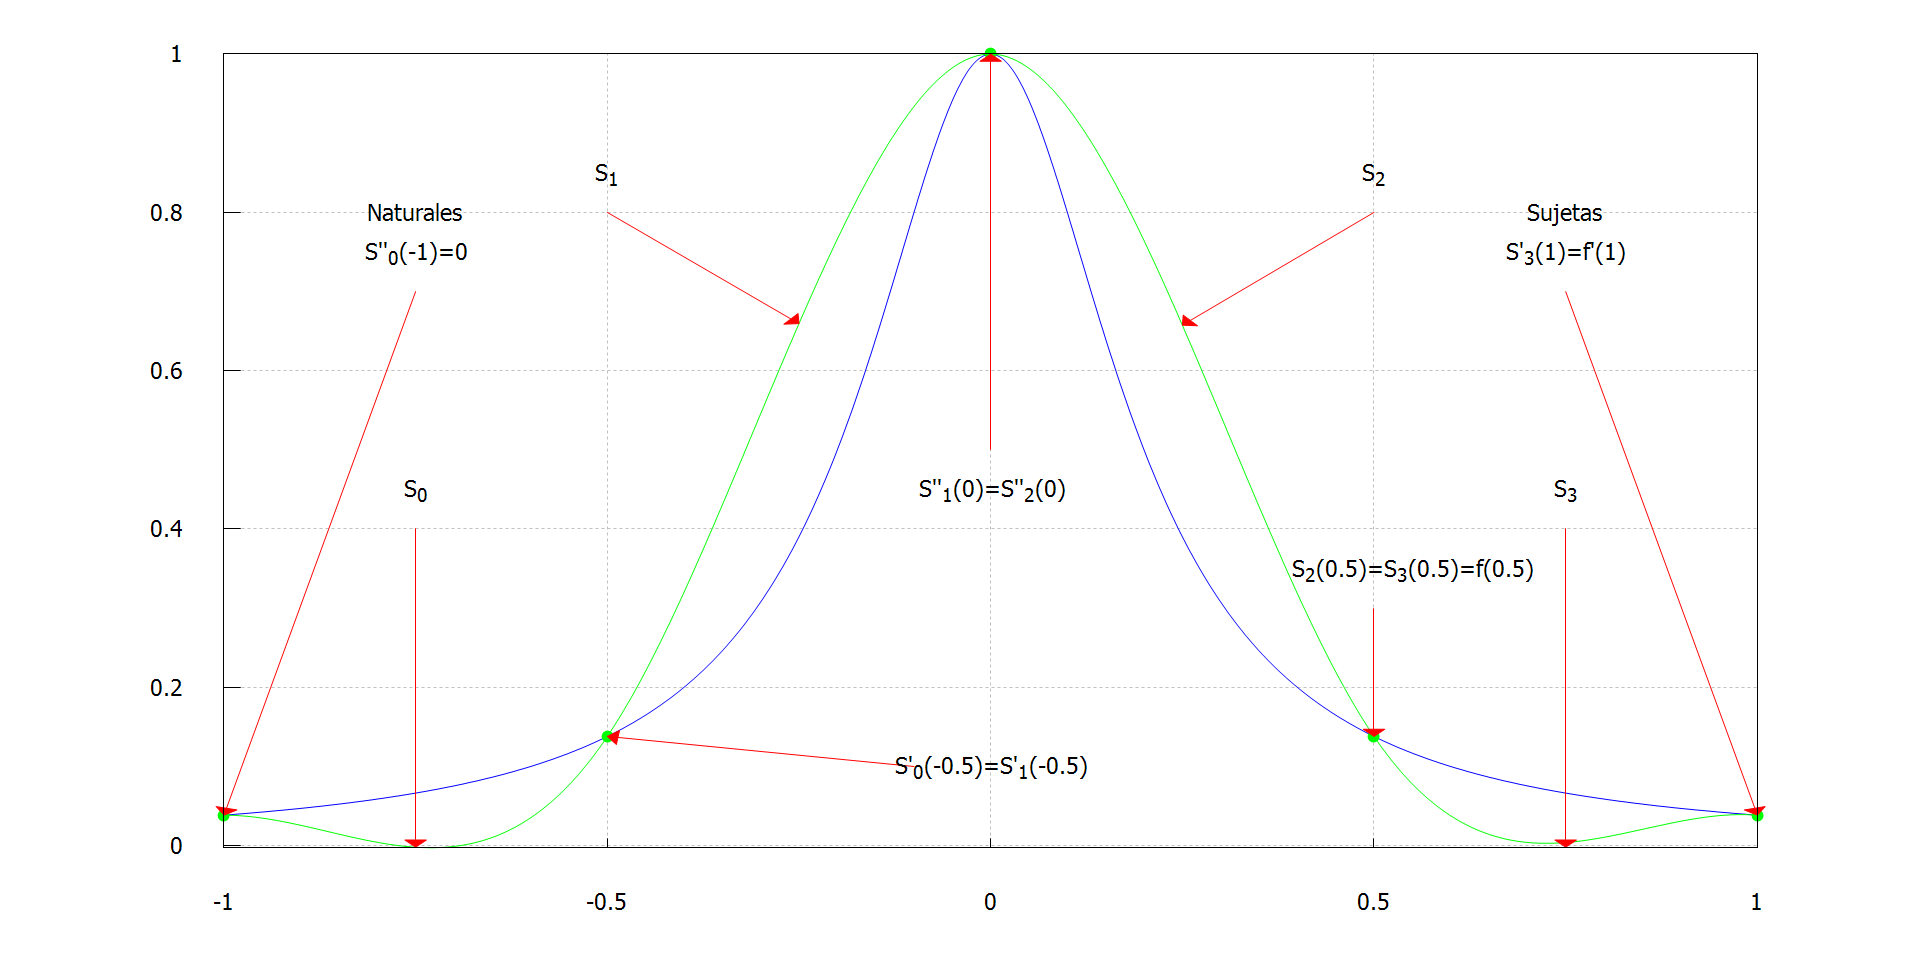
\includegraphics[scale=0.4]{Imagen22}
\end{center}
\caption{Aquí se muestran algunas condiciones de los spline. La función que se ve arriba en azul es $f(x)=\dfrac{1}{1+25x^2}$. En verde se observan los splines cúbicos.}
\end{figure}
\end{frame}
\begin{frame}[allowframebreaks]{Mínimos cuadrados}
Considere el siguiente conjunto de datos $\{(x_i,y_i)\}_{i=1}^{N}$ asociados:
\begin{displaymath}
\begin{bmatrix}
1&2&3&4&5&6&7&8&9&10\\
\downarrow &\downarrow &\downarrow &\downarrow &\downarrow &\downarrow &\downarrow &\downarrow &\downarrow &\downarrow\\
3&5&9&11&15&17&20&24&26&29
\end{bmatrix}
\end{displaymath}
Abajo se aprecian los pares ordenados correspondientes a cada par asociado:
\begin{figure}[H]
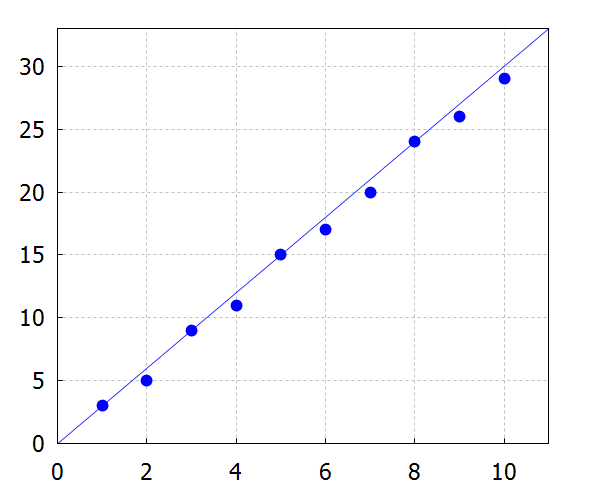
\includegraphics[scale=0.55]{Imagen2}
\caption{Recta de aproximación a los pares ordenados.}
\end{figure}
\indent El objetivo consiste en determinar la recta $Y=a_1X+a_0$ que mejor modele al conjunto de datos asociados.\\
\indent Existen algunos enfoques para encontrar esta recta:
\begin{block}{Problema Minimax}
\centering $\displaystyle \min_{a_0,a_1}\max_{1\leq i\leq 10}|y_i-(a_1x_i-a_0)|$
\end{block}
\begin{block}{Problema de desviación absoluta}
\centering $\displaystyle \min_{a_0,a_1}\sum_{i=1}^{10}|y_i-(a_1x_i-a_0)|$
\end{block}
\begin{block}{Problema de mínimos cuadrados}
\centering $\displaystyle \min_{a_0,a_1}\sum_{i=1}^{10}|y_i-(a_1x_i-a_0)|^2=\displaystyle \min_{a_0,a_1}\sum_{i=1}^{10}(y_i-(a_1x_i-a_0))^2$
\end{block}
\end{frame}
\begin{frame}{Deducción del método de mínimos cuadrados}
Defina los siguientes vectores:
$$X=[x_1,\cdots,x_n]^T$$
$$Y=[y_1,\cdots,y_n]^T$$
$$U=[1,\cdots,1]^T$$
Entonces podemos pensar en el problema de ajuste de la siguiente manera: Deseamos encontrar $a_0$ y $a_1$ tales que
$$a_1X+a_0U=Y$$
De forma matricial esto sería:
\begin{displaymath}
(X|U)
\left(
\begin{array}{c}
a_1\\
a_0
\end{array}
\right)=Y
\end{displaymath}
\end{frame}
\begin{frame}{Deducción del método de mínimos cuadrados}
Si ahora se multiplica por la transpuesta de la primer matriz, se obtine:
\begin{displaymath}
\left(
\begin{array}{c}
X^T\\
U^T
\end{array}
\right)
(X|U)
\left(
\begin{array}{c}
a_1\\
a_0
\end{array}
\right)=
\left(
\begin{array}{c}
X^T\\
U^T
\end{array}
\right)
Y
\end{displaymath}
Esto es equivalente a lo siguiente:
\begin{displaymath}
\left(
\begin{array}{cc}
X^TX &X^TU\\
U^TX & U^TU
\end{array}
\right)
\left(
\begin{array}{c}
a_1\\
a_0
\end{array}
\right)=
\left(
\begin{array}{c}
X^TY\\
U^TY
\end{array}
\right)
\end{displaymath}
Como se puede apreciar, resolviendo este sistema podemos encontrar las soluciones para los coeficientes de la regresión lineal.
\end{frame}
\begin{frame}{Generalización a ajustes de tipo polinomial.}
Ahora considere le problema siguiente: Se desan encontrar los valores $[a_m,a_{m-1},\cdots,a_0]$ de manera tal que:
$$a_mX^m+\cdots+a_1X+a_0U=Y$$
Donde $X^k=[x_1^k,\cdots,x_n^k]^T$. Nuevamente esto se puede escribir como el siguiente sistema:
\textcolor{red}{
\begin{displaymath}
(X^m|X^{m-1}|\cdots X|U)
\left(
\begin{array}{c}
a_m\\
\vdots\\
a_0
\end{array}
\right)=Y
\end{displaymath}
}
Multiplicando por la transpuesta...
\end{frame}
\begin{frame}{Generalización de ajuste  de tipo polinomial}
\begin{displaymath}
\left(
\begin{array}{c}
(X^m)^T\\
\vdots\\
(X)^T\\
U^T
\end{array}
\right)
(X^m|X^{m-1}|\cdots X|U)
\left(
\begin{array}{c}
a_m\\
\vdots\\
a_0
\end{array}
\right)=
\left(
\begin{array}{c}
(X^m)^T\\
\vdots\\
(X)^T\\
U^T
\end{array}
\right)
Y
\end{displaymath}
Lo que termina siendo equivalente a resolver el sistema:
\begin{displaymath}
\left(
\begin{array}{cccc}
(X^m)^TX^m & (X^m)^TX^{m-1} &\hdots & (X^m)^TU\\
\vdots&\vdots &&\vdots\\
(X)^TX^m&(X)^TX^{m-1}&\hdots &(X)^TU\\
U^TX^m&U^TX^{m-1}&\hdots &U^TU
\end{array}
\right)
\left(
\begin{array}{c}
a_m\\
\vdots\\
a_0
\end{array}
\right)=
\left(
\begin{array}{c}
(X^m)^TY\\
\vdots\\
(X)^TY\\
U^TY
\end{array}
\right)
\end{displaymath}
\end{frame}
\section{Derivación Numérica}
\section{Integración Numérica}
\section{Problemas de valor inicial}
\section{Problemas de valores en la frontera}
\section{Ejercicios}
\begin{frame}{Ejercicios}
\label{CriterioLimite}
\action<+->{
\begin{block}{Ejercicio (Criterio de límite)}
Encontrar el límite de la sucesión $\bigg\{n\sin\bigg(\dfrac{1}{n}\bigg)\bigg\}$
\end{block}}
\textcolor{red}{
\action<+->{Usando el criterio del límite:
\begin{align*}
\lim_{n\rightarrow \infty}n\sin(1/n)=&\lim_{n\rightarrow \infty}\dfrac{\sin(1/n)}{(1/n)}\\}
\action<+->{=&\lim_{n\rightarrow \infty}\dfrac{\cos(1/n)(-1/n^2)}{(-1/n^2)}\\}
\action<+->{=&\lim_{n\rightarrow \infty}\cos(1/n)\\}
\action<+->{=&1\\}
\end{align*}
\action<+->{Entonces el límite buscado es 1.\\}
}
\hyperlink{RetornoTeoremaPreliminares1}{\textcolor{cyan}{Teoremas Preliminares.}}
\end{frame}
\begin{frame}{Ejercicios}
\label{Sandwich}
\begin{block}{Ejercicio (Teorema del Sandwich)}
Determine el límite de la sucesión $\bigg\{\dfrac{\cos(n)}{n}\bigg\}$.
\end{block}
\pause
\textcolor{red}{
\begin{flalign*}
\action<+->{&-1\leq \cos(n) \leq 1\\}
\action<+->{\Rightarrow &\dfrac{-1}{n}\leq \dfrac{\cos(n)}{n} \leq \dfrac{1}{n}\\}
\action<+->{\Rightarrow &\lim_{n\rightarrow \infty}\dfrac{-1}{n}\leq \lim_{n\rightarrow \infty}\dfrac{\cos(n)}{n} \leq \lim_{n\rightarrow \infty}\dfrac{1}{n}\\}
\action<+->{\Rightarrow &0\leq \lim_{n\rightarrow \infty}\dfrac{\cos(n)}{n} \leq 0\\}
\end{flalign*}
\action<+->{Por lo tanto, el límite de la sucesión en cuestión es 0.\\}}
\hyperlink{RetornoTeoremaPreliminares1}{\textcolor{cyan}{Teoremas Preliminares.}}
\end{frame}
\begin{frame}{Ejercicios}
\label{ConvergenciaMonotona}
\begin{block}{Ejercicio (Teorema de la sucesión monótona)}
Encuentre el límite de la sucesión definida recursivamente por $a_n=\sqrt{1+a_{n-1}}$ con $a_1=1$, asumiendo que $\{a_n\}$ es acotada superiormente y es estrictamente creciente. 
\end{block}
\textcolor{red}{
\action<+->{Por el teorema de convergencia monótona existe el límite; sea $L$ tal límite, entonces:}
\begin{align*}
\action<+->{&a_n=\sqrt{1+a_{n-1}}\\}
\action<+->{\Rightarrow  \lim_{n\rightarrow \infty} &a_n=\lim_{n\rightarrow \infty}\sqrt{1+a_{n-1}}\\}
\action<+->{\Rightarrow  L=\ &\sqrt{1+L}\\}
\end{align*}
\action<+->{Resolviendo la última ecuación se obtiene que:
$$L=\dfrac{1+\sqrt{5}}{2}$$}
}
\hyperlink{RetornoTeoremaPreliminares1}{\textcolor{cyan}{Teoremas Preliminares.}}
\end{frame}
\begin{frame}{Ejercicios}
\label{EjercicioExtremos}
\begin{block}{Ejercicio(Teorema de valores extremos)}
Encuentre $\displaystyle\max_{x\in[2,5]}|f(x)|$ donde $f(x)=1-\exp(-\cos(x-1))$.
\end{block}
\textcolor{red}{
\begin{itemize}
\item \action<+->{$f$ es continua y diferenciable en [2,5].}
\item \action<+->{Por el teorema de valores extremos, existen $c_1$, $c_2$ tales que $$f(c_1)\leq f(x)\leq f(c_2),$$
para todo $x\in[2,5]$ y entonces $\displaystyle\max_{x\in[2,5]}|f(x)|= \max(|f(c_1)|,|f(c_2)|)$.}
\item \action<+->{Además dado que la función es diferenciable, se sabe que los posibles valores extremos se alcanzan en 2, 5 o donde la derivada se hace cero.$$f'(x)=\exp(-\cos(x-1))(\sin(x-1))=0.$$
Las soluciones de esta ecuación son $x=1+n\pi.$, $n\in\mathbb{Z}$. La única solución que se encuentra en el intervalo [2,5] es $x=1+\pi$. }
\end{itemize}
}
\end{frame}
\begin{frame}{Ejercicios}
\begin{itemize}
\item \action<+->{Al evaluar en los candidatos, se obtiene:
\begin{itemize}
\item $f(2)\approx 0.42$.
\item $f(5)\approx -0.92$.
\item $f(1+\pi)\approx -1.72$.
\end{itemize}
Entonces $c_1=1+\pi$ y $c_2=2$.
}
\item \action<+->{De lo anterior se obtiene que $\displaystyle\max_{x\in[2,5]}|f(x)|= \max(|f(2)|,|f(1+\pi)|)=e-1.$}
\end{itemize}
\action<+->{
\begin{figure}[H]
\begin{center}
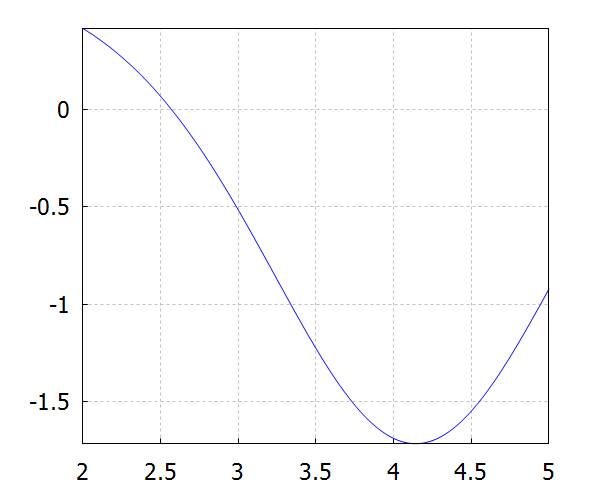
\includegraphics[scale=0.5]{Imagen16}
\end{center}
\caption{Gráfica de $f(x)$ en [2,5].}
\end{figure}}
\hyperlink{RetornoTeoremaPreliminares3}{\textcolor{cyan}{Teoremas Preliminares.}}
\end{frame}
\begin{frame}{Ejercicios}
\label{EjercicioIntermedio}
\action<+->{
\begin{block}{Ejercicio (Teorema del valor intermedio)}
Determine si la siguiente ecuación tiene una solución
$$\sin(x)/\log(x)=0,$$
en el intervalo $[2,4]$.
\end{block}}
\textcolor{red}{
\action<+->{
Elija $f(x)=\sin(x)/\log(x)$.\\ 
\indent Dado que $f(2)>0$, $f(4)<0$, $f$ es continua en [2,4] y $f(4)<0<f(2)$, entonces (tomando $K=0$) por el teorema del valor intermedio existe un $c$ tal que $f(c)=K=0$.\\}
}
\hyperlink{RetornoTeoremaPreliminares4}{\textcolor{cyan}{Teoremas Preliminares.}}
\end{frame}
\begin{frame}[fragile]{Ejercicios}
\label{EjercicioBiseccion}
\begin{block}{Ejercicio(Método de bisección)}
Encuentre la aproximación para la solución del problema anterior usando el método de bisección. Además determine cuál es el valor de $n$ para conseguir un error de a lo mucho $10^{-5}$; calcule el error asumiendo que la solución exacta es $\pi$. ($f(x)=\sin(x)/\log(x)$, $x\in[2,4].$)
\end{block}
\small
\begin{lstlisting}[style=mystyle,backgroundcolor=\color{gray!30}]
n     a       b       p       f(p)            |p-p*|
0     2       4       *       *               *
1     3       4       3       1.284530e-01    1.415927e-01
2     3       3.5     3.5     -2.800077e-01   3.584073e-01
3     3       3.25    3.25    -9.179542e-02   1.084073e-01
...
16    3.1416  3.1416  3.1416  1.887677e-05    2.160867e-05
17    3.1416  3.1416  3.1416  5.547064e-06    6.349879e-06
18    3.1416  3.1416  3.1416  -1.117744e-06   1.279516e-06
19    3.1416  3.1416  3.1416  2.214656e-06    2.535182e-06
\end{lstlisting}
\normalsize
\pause
\textcolor{red}{Se necesita garantizar que $|p-\pi|\leq 10^{-5}$. Por el teorema de bisección, se tiene $$|p-\pi|\leq \dfrac{b-a}{2^n}=\dfrac{4-2}{2^n}=\dfrac{1}{2^{n-1}}\leq 10^{-5}$$
Si se resuleve la última desigualdad, se obtiene que $n\geq 17.61$, es decir que se puede escoger $n=18$.}\hyperlink{RetornoTeoremaRaices1}{\textcolor{cyan}{Raices de ecuaciones.}}
\end{frame}
\begin{frame}{Ejercicios}
\action<+->{
\begin{block}{Ejercicio (Teorema de Taylor)}
Considere la función $f(x)=\ln(\ln(x))$. Determine lo siguiente:
\begin{itemize}
\item Calcule $P_3(x)$ centrada en $x_0=3$.
\item Aproxime $P_3(1.5).$
\item Encuentre la expresión para $R_3(x)$.
\item Calcule el error absoluto y relativo de la aproximación anterior.
\item Aproxime $\displaystyle \int_{2}^{4}f(x)dx$ usando $P_3(x)$.
\end{itemize}
\end{block}
}
\label{EjercicioTaylor}
\textcolor{red}{
\begin{align*}
\action<+->{P_3(x)=&\displaystyle \sum_{k=0}^{3}\dfrac{f^{(k)}(x_0)}{k!}(x-x_0)^k\\}
\action<+->{=&\dfrac{f(3)}{0!}(x-3)^0+\dfrac{f'(3)}{1!}(x-3)^1+\dfrac{f''(3)}{2!}(x-3)^2+\dfrac{f'''(3)}{3!}(x-3)^3.}
\end{align*}}
\end{frame}
\begin{frame}{Ejercicios}
\textcolor{red}{
\begin{align*}
\action<+->{=&\ln(\ln(3))+\dfrac{(x-3)}{3\ln(3)}-\bigg(\dfrac{1}{18\ln(3)}+\dfrac{1}{18\ln^2(3)}\bigg)(x-3)^2\\
&+\dfrac{1}{162}\bigg(\dfrac{2}{\ln(3)}+\dfrac{3}{\ln^2(3)}+\dfrac{2}{\ln^3(3)}\bigg)(x-3)^3}
\end{align*}
}
\textcolor{blue}{
\begin{align*}
\action<+->{P_3(1.5)=&\ln(\ln(3))+\dfrac{(1.5-3)}{3\ln(3)}-\bigg(\dfrac{1}{18\ln(3)}+\dfrac{1}{18\ln^2(3)}\bigg)(1.5-3)^2\\
&+\dfrac{1}{162}\bigg(\dfrac{2}{\ln(3)}+\dfrac{3}{\ln^2(3)}+\dfrac{2}{\ln^3(3)}\bigg)(1.5-3)^3\\
\approx & -0.69955228}
\end{align*}
}
\textcolor{red}{
\begin{align*}
\action<+->{R_3(x)=&\dfrac{f^{(4)}(\xi(x))}{(4)!}(x-3)^{4}\\
=&-{{6\,\left(\log \xi\left(x\right)\right)^3+11\,\left(\log \xi
 \left(x\right)\right)^2+12\,\log \xi\left(x\right)+6}\over{\xi\left(
 x\right)^4\,\left(\log \xi\left(x\right)\right)^4}}(x-3)^4.
}
\end{align*}
}
\end{frame}
\begin{frame}{Ejercicios}
Observación: Si $p^*$ es una aproximación de $p$, entonces se definen los errores:
\begin{itemize}
\item Error absoluto: $|p-p^*|$.
\item Error relativo: $\dfrac{|p-p^*|}{|p|}$.
\end{itemize}
\textcolor{blue}{Error absoluto:
\begin{align*}
\action<+->{|f(1.5)-P_3(1.5)|\approx & 0.20316817}
\end{align*}
}
\textcolor{red}{Error relativo:
\begin{align*}
\action<+->{\dfrac{|f(1.5)-P_3(1.5)|}{|f(1.5)|}\approx &  0.22506211}
\end{align*}
}
\end{frame}
\begin{frame}{Ejercicios}
\textcolor{blue}{
\begin{align*}
\action<+->{\displaystyle \int_{2}^{4}f(x)dx\approx &\displaystyle \int_{2}^{4}P_3(x)dx\\}
\action<+->{=&\displaystyle \int_{2}^{4}\ln(\ln(3))+\dfrac{(x-3)}{3\ln(3)}-\bigg(\dfrac{1}{18\ln(3)}+\dfrac{1}{18\ln^2(3)}\bigg)(x-3)^2\\
&+\dfrac{1}{162}\bigg(\dfrac{2}{\ln(3)}+\dfrac{3}{\ln^2(3)}+\dfrac{2}{\ln^3(3)}\bigg)(x-3)^3 dx\\}
\action<+->{=&\bigg[\displaystyle \ln(\ln(3))(x-3)+\dfrac{(x-3)^2}{6\ln(3)}-\bigg(\dfrac{1}{54\ln(3)}+\dfrac{1}{54\ln^2(3)}\bigg)(x-3)^3\\
&+\dfrac{1}{162}\bigg(\dfrac{2}{4\ln(3)}+\dfrac{3}{4\ln^2(3)}+\dfrac{2}{4\ln^3(3)}\bigg)(x-3)^4\bigg]_{2}^{4}\\}
\action<+->{&\approx 0.1242167}
\end{align*}
}
\hyperlink{RetornoTeoremaPreliminares5}{\textcolor{cyan}{Teoremas Preliminares.}}
\end{frame}
\begin{frame}[fragile]{Ejercicios}
\label{EjercicioNewton}
\begin{block}{Ejercicios (Método de Newton-Raphson,Examen I, PACI2023)}
Una partícula parte del reposo sobre un plano inclinado uniforme, cuyo ángulo $\theta$ cambia con una rapidez constante de $\dfrac{d\theta}{dt}=\omega<0$.\\
Al final de $t$ segundos, la posición del objeto está dada por:
$$x(t)=-\dfrac{g}{2\omega^2}\bigg(\dfrac{e^{\omega t}-e^{-\omega t}}{2}-\sin(\omega t)\bigg)$$
Suponga que la partícula se desplazó 60 pies en 2s. Encuentre la rapidez $\omega$ con que cambia $\theta$. Asuma que $g=32.17 pies/s^2$. Para calcular dicha rapidez realice lo siguiente:
\end{block}
\begin{itemize}
\item\action<+->{Plantee la ecuación y determine el intervalo con extremos enteros de menor valor absoluto que contenga la solución de la ecuación.\\}
\action<+->{\textcolor{red}{Dado que $x(2)=60$, se sustituye esto en la ecuación ofrecida.}}
\end{itemize}
\end{frame}
\begin{frame}{Ejercicios}
\action<+->{\textcolor{red}{$$60=-\dfrac{g}{2\omega^2}(\sinh(2\omega)-\sin(2\omega))$$
$$120+\dfrac{g}{\omega^2}(\sinh(2\omega)-\sin(2\omega))=0$$
Defina entonces:
$$f(\omega)=120+\dfrac{g}{\omega^2}(\sinh(2\omega)-\sin(2\omega)).$$}}
\action<+->{\textcolor{red}{Dado que $\omega<0$, entonces rápidamente se puede ver que $f(-1)>0$ y $f(-2)<0$. Con esto se escoge el intervalo $[-2,-1]$.}}
\begin{itemize}
\item \action<+->{¿Cuántas iteraciones son suficientes para alcanzar una exactitud de $10^{-12}$ mediante el método de bisección?}\\
\action<+->{\textcolor{blue}{Usando el teorema de cota de error del método de bisección se plantea:
\begin{align*}
|p_n-p|\leq & \dfrac{b-a}{2^n}=\dfrac{-1-(-2)}{2^n}=\dfrac{1}{2^n}\leq 10^{-12}.\\
10^{12}\leq & 2^n.
\end{align*}
Resolviendo la inecuación se obtiene $n\geq 40$.
}}
\end{itemize}
\end{frame}
\begin{frame}[fragile]{Ejercicios}
\begin{itemize}
\action<+->{\item Realice tres iteraciones del método de bisección, calcule el error relativo en cada iteración.\\}
\action<+->{\textcolor{red}{Cuando no conocemos el valor de la raíz, la estimación del error relativo se calcula de la siguiente forma:
$$\dfrac{|p_{n+1}-p_n|}{|p_{n+1}|}$$
De esta forma se puede generar la siguiente tabla:
}
}
\end{itemize}
\pause
\small
\begin{lstlisting}[style=mystyle,backgroundcolor=\color{gray!30}]
n     a       b       p      f(p)          Error relativo
0     -2      -1      *      *             *
1     -1.5    -1      -1.5   -2.121565e+01 *
2     -1.5    -1.25   -1.25  7.755373e+00  2.000000e-01
3     -1.375  -1.25   -1.375 -6.045842e+00 9.090909e-02
\end{lstlisting}
\normalsize
\begin{itemize}
\action<+->{\item Aplique el método de Newton-Raphson para obtener una aproximación con una exactitud de $10^{-5}$. Utilice como aproximación inicial la aproximación encontrada en el iniciso anterior.}
\end{itemize}
\end{frame}
\begin{frame}[fragile]{Ejercicios}
\small
\begin{lstlisting}[style=mystyle,backgroundcolor=\color{gray!30}]
n      p_n     f(p_n)         Error relativo
0      -1.375  -6.0458        *
1      -1.3226 -1.150768e-01  3.962162e-02
2      -1.3216 -4.145716e-05  7.840103e-04
3      -1.3216 -5.371703e-12  2.826484e-07
\end{lstlisting}
\normalsize
\textcolor{blue}{Primero se requiere calcular la derivada de la función analizada:
$$f'(\omega)={{32.17\,\left(2\,\cosh \left(2\,\omega\right)-2\,\cos \left(2\,\omega\right)
 \right)}\over{\omega^2}}-{{64.34\,\left(\sinh \left(2\,\omega\right)-\sin
 \left(2\,\omega\right)\right)}\over{\omega^3}}$$
 Con esto la iteración del método de Newton queda expresado como:
 \small
 \begin{align*}
 p_{n+1}=&p_{n}-\dfrac{f(p_n)}{f'(p_n)}\\
 =&p_n+\\
 &{{3217\,p_{n}\,\sinh \left(2\,p_{n}\right)-3217\,p_{n}\,\sin
 \left(2\,p_{n}\right)+12000\,p_{n}^3}\over{6434\,\sinh \left(2\,p_{n
 }\right)-6434\,\sin \left(2\,p_{n}\right)-6434\,p_{n}\,\cosh \left(2
 \,p_{n}\right)+6434\,p_{n}\,\cos \left(2\,p_{n}\right)}}
 \end{align*}
 \normalsize
 Para los resultados se uso el error relativo, es decir $\dfrac{|p_{n+1}-p_{n}|}{|p_{n+1}|}$.\\
}
\hyperlink{RetornoTeoremaRaices4}{\textcolor{cyan}{Raices de ecuaciones.}} 
\end{frame}
\begin{frame}[fragile]{Ejercicios}
\label{EjercicioNewtonSistemas}
\begin{block}{Ejercicio (Ecuaciones no lineales, Ejercicio IIPAC2023)}
Sea el sistema de ecuaciones no lineales:
\begin{displaymath}
\begin{bmatrix}
\ln(x^2+y^2)-\sin(xy) &=& \ln(2)-\ln(\pi)\\
x^2+4y^2\cos(x) &=&4
\end{bmatrix}
\end{displaymath}
Realice una iteración del método de Newton Raphson para sistemas con la aproximación inicial:
\begin{displaymath}
p_0=\begin{bmatrix}
-1.5\\
-2.5
\end{bmatrix}
\end{displaymath}
Además calcule $\parallel p_k-p_{k-1}\parallel_{\infty}$ y $\parallel p_k-p_{k-1}\parallel_2$.
\end{block}\pause
\textcolor{red}{
Primero se definirán la función y el jacobiano para usar el método de Newton:
\small
\begin{displaymath}
F(x,y)=\begin{pmatrix}
\ln(x^2+y^2)-\sin(xy)+\ln(\pi)-\ln(2)\\
4\cos(x)y^2+x^2-4\\
\end{pmatrix}
\end{displaymath}
}
\end{frame}
\begin{frame}[fragile]{Ejercicios}
\small
\textcolor{red}{
\begin{align*}
J(x,y)=&\begin{pmatrix}
\dfrac{2x}{x^2+y^2}-y\cos(xy) & \dfrac{2y}{x^2+y^2}-x\cos(xy)\\
2x-4\sin(x)y^2 & 8 \cos(x)y 
\end{pmatrix}\\
J(-1.5,-2.5)=&
\begin{pmatrix}
 - 2.40433956981949  & - 1.819074330126988\\
 21.93737466510136   & - 1.414744033354058
\end{pmatrix}\\
J^{-1}(-1.5,-2.5)=&
\begin{pmatrix}
-0.03266761001938535 &  0.04200393103760224\\
-0.5065521278147188 &  - 0.05551818955887632
\end{pmatrix}\\
F(-1.5,-2.5)=&
\begin{pmatrix}
0.873750\\
0.018430
\end{pmatrix}\\
p_1=&p_0-J^{-1}(p_0)F(p_0)\\
=&
\begin{pmatrix}
-1.5\\
2.5
\end{pmatrix}
-J^{-1}(-1.5,-2.5)F(-1.5,-2.5)=
\begin{pmatrix}
-1.472231\\
-2.056377
\end{pmatrix}
\end{align*}}
\small
\begin{lstlisting}[style=mystyle,backgroundcolor=\color{gray!30}]
n  p_n(1)  p_n(2)  f(p_n)        Norma 2       Norma inf
0  -1.5    -2.5    0.87375       *             *
1  -1.4722 -2.0564 -9.606503e-02 4.444916e-01  4.436233e-01
2  -1.4663 -2.1091 -1.654021e-04 5.303760e-02  5.270221e-02
3  -1.4667 -2.1087 -1.031003e-07 5.406173e-04  3.834635e-04
\end{lstlisting}
\normalsize
\hyperlink{RetornoTeoremaRaices10}{\textcolor{cyan}{Raices de ecuaciones.}} 
\end{frame}
\begin{frame}{\textbf{Referencias}}
\printbibliography
\end{frame}
\end{document}